\section{Irradiador $\beta$-$\gamma$}
Para realizar ensayos con radiación,
construímos un aparato que nos permite exponer dispositivos a rayos $\beta$ y
$\gamma$ de manera segura para el operario y controlando la dosis con precisión.
Este aparato consiste en un tubo de plomo con una capa de PVC en su pared
interior (\figref{fig:corteirradiador}).
\fig{corteirradiador}{figuras/poster/corte.pdf}{Corte del irradiador.}

Todas las superficies donde puede impactar una partícula $\beta$ tienen una
capa de plástico,
para frenar la partícula con la menor producción posible de
radiación X de frenado.

En un extremo de la cavidad se encuentra una pastilla de \Strontium 
(\figref{fig:fuente})
\fig{fuente}{figuras/poster/fuente.pdf}{Corte de la fuente $\beta$.}
colocada en una mochila de plástico unida a un bloque de plomo giratorio
(\figref{fig:piezagiratoria}).
\fig{piezagiratoria}{figuras/poster/piezagiratoria.png}
{Detalle de la pieza giratoria donde se coloca la fuente $\beta$.}
En una orientación de este bloque,
el mismo se interpone entre la fuente radioactiva y el interior de la cavidad.
Esto permite abrir la cavidad para manipular sus contenidos con seguridad
(\figref{fig:posicionno}).
En la posición de irradiar, la fuente emite partículas $\beta$ hacia el interior
(\figref{fig:posicionsi}).

Gracias al trabajo de Laboratorio 6 y 7 de Javier Badía,
el movimiento de la fuente está motorizado.
Esto permite girar la fuente con un interruptor de manera fácil, rápida y repetible.
\begin{figure}[H]
    \centering
    \begin{subfigure}[b]{.45\textwidth}
        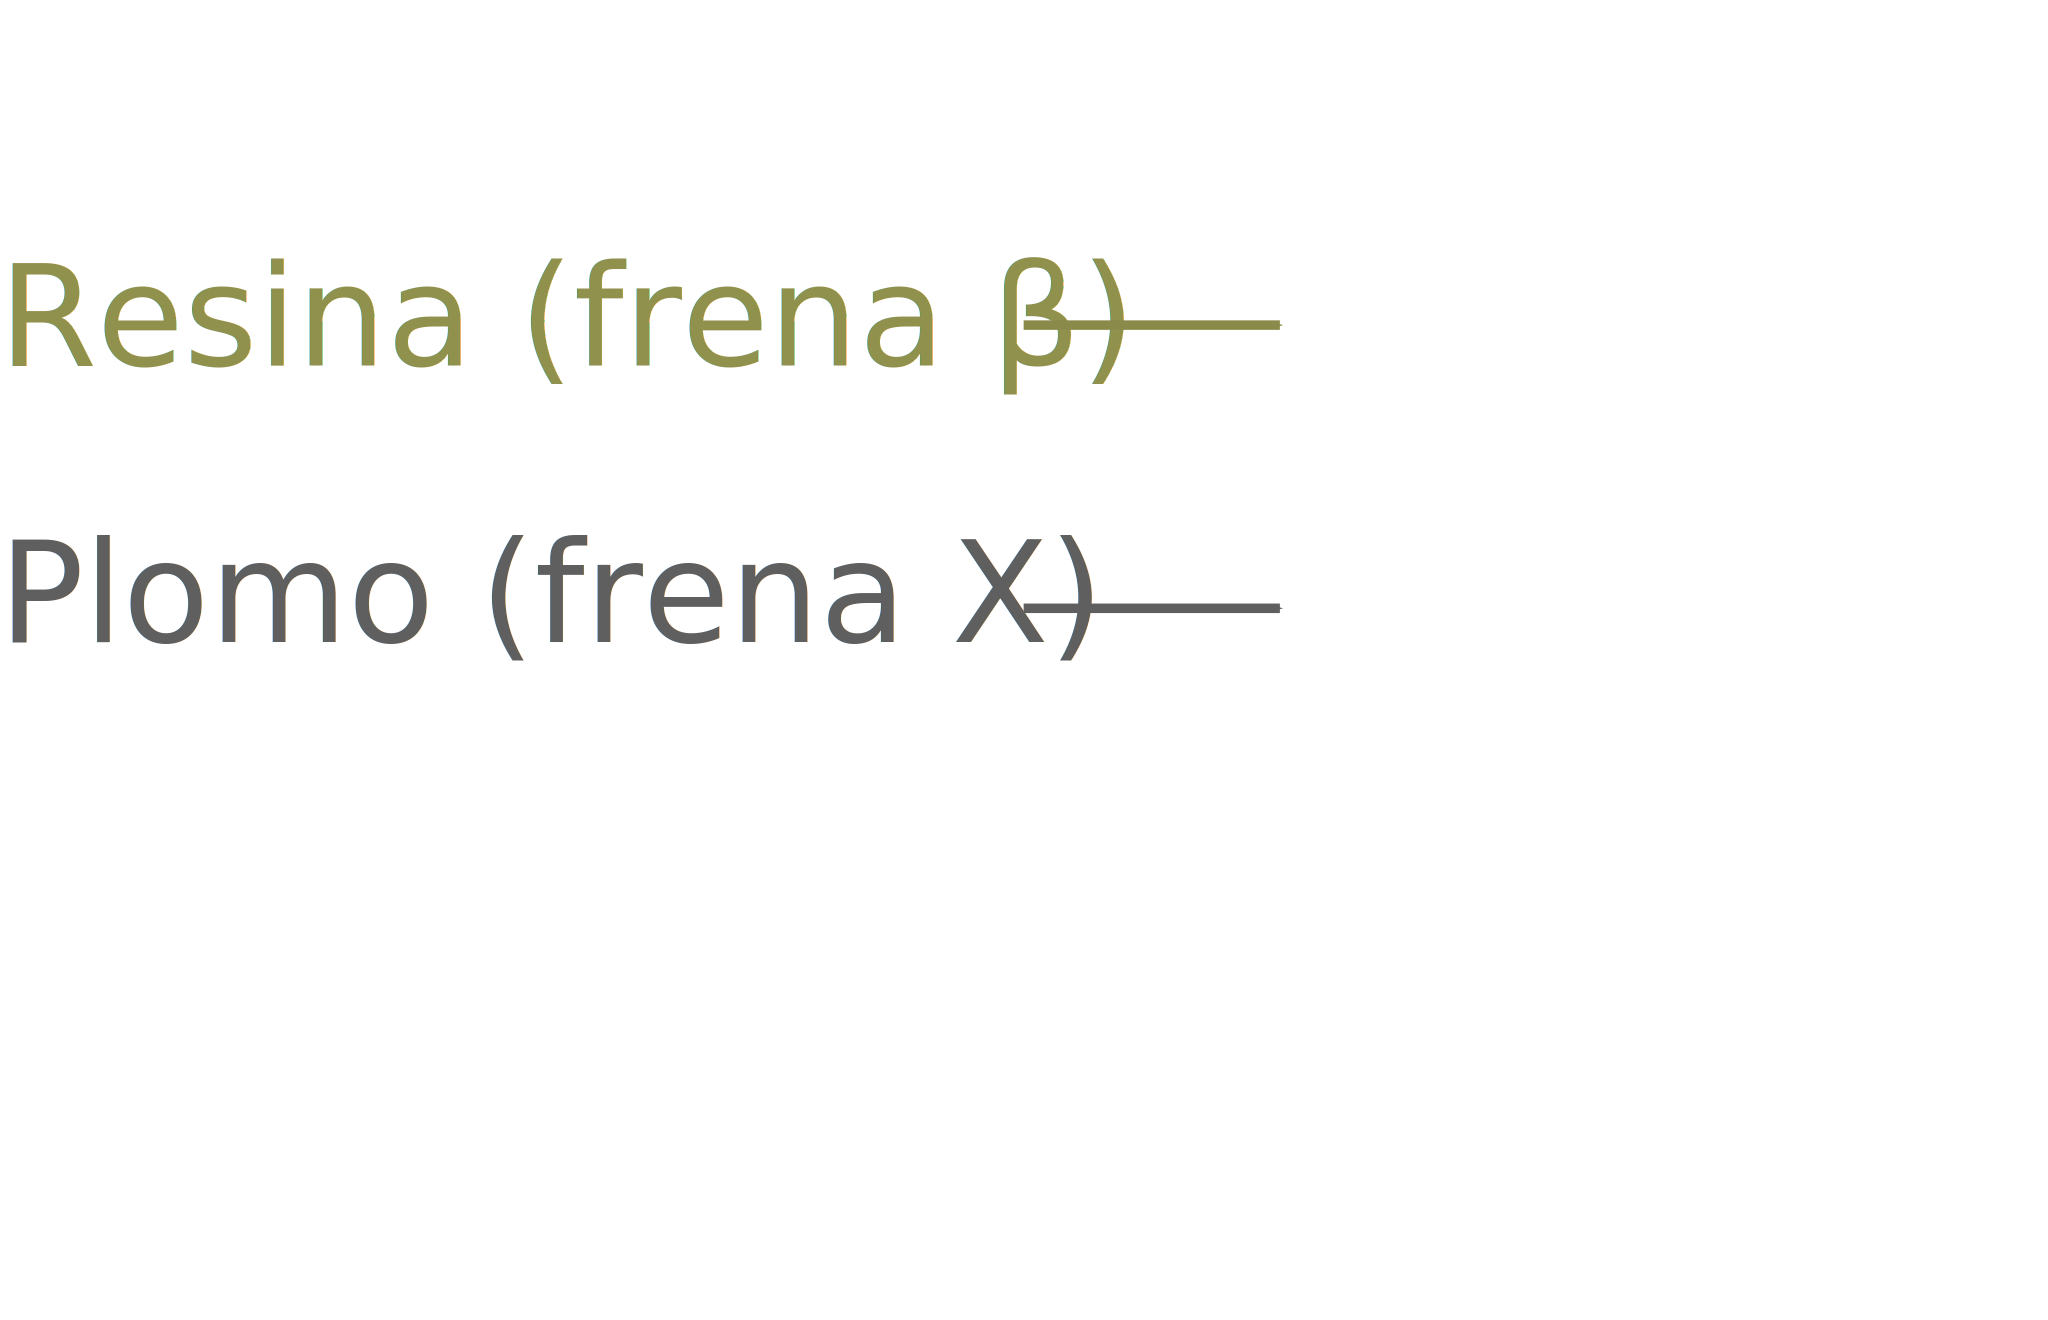
\includegraphics{figuras/poster/posicion_no.png}
        \caption{Posición segura.}
        \label{fig:posicionno}
    \end{subfigure}
    \hspace{5mm}
    \begin{subfigure}[b]{.45\textwidth}
        \includegraphics{figuras/poster/posicion_si.png}
        \caption{Posición para irradiar.}
        \label{fig:posicionsi}
    \end{subfigure}
    \caption{Posiciones de la pieza giratoria.}
    \label{fig:posicionespieza}
\end{figure}
\subsection{Construcción}
\subsubsection{Paredes}
Cubrimos ambos extremos de la cavidad con discos de acrílico
de \SI{10}{\milli\meter} de espesor y \SI{90}{\milli\meter} de diámetro.

Para los laterales consideramos moldear tubos de parafina o acrílico
debido a la dificultad de conseguir tubos de PVC con paredes de
\SI{10}{\milli\meter}.
Finalmente optamos por usar un tubo interior y uno exterior de PVC,
y rellenar el espacio intermedio con acrílico.
\subsubsection{Pieza giratoria}
La pieza giratoria está hecha de plomo fundido y luego mecanizado
(\figref{fig:construccion_mariposa}).
\fig{construccion_mariposa}{figuras/irradiador/construccion_mariposa.pdf}
{Pasos para la fabricación de la pieza giratoria de plomo.
El torneado requiere un lugar de donde agarrar a la pieza,
que luego cortamos.}
Para la fundición recurrimos a Abraham Murillo en la 
Escuela Técnica Nº 33 Fundicion Maestranza del Plumerillo. 
Allí tornearon una forma de madera con las dimensiones aproximadas de la pieza final.
La hicimos un poco más grande que las dimensiones finales tomando en cuenta
\begin{itemize}
    \item la contracción del plomo al enfriarse, y
    \item el margen de material extra necesario para tornear.
\end{itemize}
Rodeamos esta forma con tierra apisonada para crear un molde.
El mismo cuenta con un tubo para verter el metal fundido 
y un agujero para ventear gases
(\figref{fig:moldeplomo}).
\fig{moldeplomo}{figuras/irradiador/molde_plomo.pdf}
{Corte del molde usado para fundir la pieza giratoria de plomo.
Está hecho de tierra apisonada alrededor de una forma de madera.
Vertimos el plomo fundido por el tubo de la derecha.
El agujero superior sirve para ventear gases.}
La pieza que sale de este proceso tiene una superficie rugosa
debido a los granos de la tierra usada para el molde.
Para darle una terminación lisa y las dimensiones exactas que necesitamos,
recurrimos a Eriel Fernandez del taller mecánico de FIUBA.
La idea original era darle forma esférica,
pero descartamos esta idea debido a la dificultad
de tornear una esfera en un torno manual.
En cambio, optamos por una forma fácil de tornear
pero que obture lo más posible la cavidad del irradiador 
y pueda girar dentro de la misma
(\figref{fig:torneo_simple}).
\fig{torneo_simple}{figuras/irradiador/torneo_simple.pdf}
{Elegimos una forma simple de tornear que obture lo más posible 
la cavidad del irradiador y pueda girar en su interior.
Para eso nos aseguramos de que las esquinas no se salgan de un círculo
con el diámetro interior de la cavidad.}
Las dimensiones finales están en la \figref{fig:torneo}.
La blandez del plomo demandó un torneado cuidadoso a bajas revoluciones.
\fig{torneo}{figuras/irradiador/torneo.pdf}
{Corte lateral de la pieza giratoria de plomo luego del torneado
(dimensiones en mm).}
\subsubsection{Mochila de la fuente}
La fuente va colocada en una pieza de plástico.
Si bien la fuente cuenta con un agujero roscado,
fijarla con un tornillo requiriría manipularla de cerca,
exponiendo las manos a radiación durante cierto tiempo.
Por eso decidimos montarla en un bolsillo donde se puede 
rápidamente dejar caer la fuente,
minimizando la exposición del que realice la tarea.

Quisimos asegurarnos de que el plástico frene todos los electrones antes de llegar a
la pieza de plomo. 
Para eso le dimos una forma redonda que cubra lo más posible al plomo,
con la restricción de que pueda girar en la cavidad.

Debido a la dificultad de moldear esta forma (redonda y con una cavidad)
en resina, recurrimos a Iván G. Pollitzer y el 
Laboratorio Abierto de Electrónica de FIUBA.
Iván nos guió en el diseño de una pieza impresa en 3D en ABS.
Esta pieza consiste en dos partes impresas por separado
(\figref{fig:blender}),
\fig{blender}{figuras/irradiador/blender_small.png}
{Las dos partes que imprimimos en 3D en ABS y pegamos para formar la montura de
    la fuente.
Entre las dos partes queda un bolsillo donde se coloca la fuente.}
que luego rellenamos de acrílico y unimos.

Unimos la mochila de plástico a la pieza de plomo usando tornillos sin cabeza,
agujereando y roscando ambas piezas.
\subsection{Cálculos de protección}
\subsubsection{Frenado $\beta$}
% FIXME: repetido, todo esto está en la sección anterior
Usamos PVC para el frenado de electrones, porque está disponible en tubos
del tamaño requerido.
Tiene baja eficiencia radiativa y el rango de nuestros electrones más
energéticos en PVC es inferior a \SI{1}{\centi\meter}.
Por las mismas razones construimos las tapas del cilindro con discos de
acrílico de \SI{1}{\centi\meter} de espesor,
pegados a las tapas de plomo.
La mochila donde montamos la fuente consiste de plástico ABS 
extruído en una impresora 3D en el LABi.
Esto requirió separar el modelo inicial en dos partes que fueron pegadas y
terminadas con herramientas manuales.
%
\subsubsection{Cálculos de radiación de frenado}
Las partículas $\beta$ de la fuente empiezan a frenarse en el plástico,
donde producen radiación X de frenado.
Estimamos su magnitud partiendo del espectro de energía de los
electrones emitidos por la fuente.
Dado que está en equilibrio secular 
(misma actividad de \Strontium y de \Yttrium),
sumamos sus espectros provenientes de 
Radiological Toolbox\cite{eckerman2006radiological}
y normalizamos a la actividad nominal de la fuente, \SI{100}{\milli\curie}
(\figref{fig:actividadsr90}).
\fig{actividadsr90}{figuras/irradiador/actividad.pdf}
{Espectro de electrones provenientes de una fuente de
\Strontium con actividad \SI{100}{\milli\curie}\cite{eckerman_icrp_2007}.}
Luego calculamos el espectro de bremsstrahlung integrando la \equref{eq:kramers}
(\figref{fig:espectrox}).
\fig{espectrox}{figuras/irradiador/espectrox.pdf}
{Espectro de bremsstrahlung calculado en la cara exterior del PVC.}
%
\subsubsection{Atenuación de rayos X en el plomo}
Aplicamos la \equref{eq:absorcionx} 
usando tasas de absorción en plomo tabuladas por NIST\cite{xraycoef},
resultando en el espectro atenuado de la \figref{fig:xatenuado}
\fig{xatenuado}{figuras/irradiador/xatenuado.pdf}
{Espectro de rayos X calculado en la cara exterior del irradiador.}
% TODO: tasa de dosis final según distancia, comparar con mediciones
%
%
\subsubsection{Cálculos Monte-Carlo de fuente de \Strontium}
La fuente de \Strontium  emite electrones con un espectro amplio de
energías (\figref{fig:actividadsr90}).
Este consiste en la suma del espectro de emisión de \Strontium
y el de \Yttrium.
Simulamos un haz de electrones con este espectro incidiendo normalmente sobre
tejido blando, registrando la energía que depositan en función de la
profundidad (\figref{fig:deposicionsr90}).
\fig{deposicionsr90}{figuras/montecarlo/deposicion_sr90.pdf}
{Energía depositada en tejido blando en función de la distancia,
promediando entre electrones provenientes de una fuente de \Strontium.}
Así ajustamos una potencia de frenado de masa promedio $S/\rho$ (\figref{fig:stoppingsr90})
\fig{stoppingsr90}{figuras/montecarlo/stopping_sr90.pdf}
{Potencia de frenado promedio del tejido blando para electrones provenientes de
una fuente de \Strontium.
La cruz marca que a una profundidad de \SI{0.35}{\milli\meter} la tasa de dosis 
coincide con la tabulada en \cite{delacroix_radionuclide_2002}.}
que permite calcular tasa de dosis superficial mediante
\begin{align*}
    \dot D &= \frac{AS/\rho}{4\pi r^2}
\end{align*}
con $A=\SI{100}{\milli\curie}$ la actividad de la fuente.
La tasa de dosis calculada de este modo es comparable con la tabulada en
\cite{delacroix_radionuclide_2002} si se promedia hasta una profundidad de
\SI{.35}{\milli\meter}.
Esto sirve como verificación de que nuestras simulaciones Monte-Carlo producen
valores compatibles con los que se encuentran en la literatura.
\subsubsection{Cálculos Monte-Carlo del irradiador}
Buscamos una cota superior de la tasa de dosis fuera del irradiador.
Esto brinda la mayor confianza en que su operación no es peligrosa.
Ya que el espesor del plomo es de varias longitudes características de
atenuación ($1/\mu$),
sólo pasa una fracción muy pequeña de la radiación inicial.
Por lo tanto, hay que simular la emisión de 
muchos electrones de la fuente de \Strontium
para que llegue una cantidad apreciable de radiación a la cara exterior.
Así podemos estimar de forma precisa la tasa de dosis.

Una forma de reducir el tiempo de CPU necesario para simulaciones
es usar reducción de la varianza\cite{dressel_geometrical_2003}.
Esta es una técnica para cálculos Monte Carlo que introduce un sesgo en la
evolución de la partícula.
Por ejemplo, podemos aumentar la probabilidad de que una partícula atraviese
el plomo sin interactuar, en vez de scatterear.
Llevando la cuenta de cuan improbable es la historia de la partícula,
le damos un peso menor en la estadística final.
Esto concentra la simulación en darnos muchos eventos que nos interesan
(lo cual reduce la varianza de la estimación),
minimizando la capacidad de procesamiento necesaria.

Dada la dificultad de implementar reducción de la varianza en Geant4,
optamos por acelerar el cálculo simplificando la geometría.
Simulamos un irradiador con simetría esférica,
que consiste en un cascarón de \SI{10}{\milli\meter} de acrílico rodeado por
\SI{36}{\milli\meter} de plomo (\figref{fig:corte_esferico}). 
\fig{corte_esferico}{figuras/irradiador/corte_esfera.png}
{Corte de la geometría simplificada que se usó para simular el irradiador en
Geant4.}
Toda partícula en el irradiador tiene que atravesar al menos ese espesor de
acrílico y plomo.
Por lo tanto, la dosis real va a ser aún menor a la simulada.
Dada la simetría del problema, no tenemos en cuenta la distribución en
$\theta$ y $\phi$ sino que promediamos sobre ambas variables.
Esto reduce enormemente el número de eventos necesarios para una buena
estimación de la tasa de dosis.
El resultado se ve en la \figref{fig:dosis_irradiador}.
\fig{dosis_irradiador}{figuras/montecarlo/dosis_irradiador.pdf}
{Perfil de deposición de energía en la simulación Monte-Carlo del irradiador.}
La dosis en la cara exterior del irradiador es
de \SI{20.3}{\milli\sievert} por año.
Este valor es aceptable si se tiene en cuenta que,
en condiciones reales, se toca el irradiador durante intervalos muy cortos
y el resto del tiempo se está a distancias mucho mayores.
